\documentclass[14pt, a4paper]{article}
\usepackage[utf8]{inputenc}
\usepackage[russian]{babel}
\usepackage{graphicx}
\usepackage{listings}

\title{\textbf{Отчет о выполнении лабы по флоатам}}
\author{Калашников Михаил, Б03-205}
\date{}

\begin{document}

\maketitle


\begin{enumerate}
\setcounter{enumi}{-1}

\item unsigned int $\rightarrow$ binary

\begin{lstlisting}[language=C++, basicstyle=\small]
void print_bin(unsigned int x) {
	unsigned int y;
	
	y = -1;
	y >>= 1;
	y++;
	
	for (int i = 1; i < 33; i++) {
		cout << ((x & y) != 0);
		y >>= 1;
		
		if (i % 8 == 0) {
			cout << ' ';
		} 
	}
}
\end{lstlisting}

Данная функция выводит в терминал побитовое разложение числа путем сравнения каждой ячейки памяти, занятой числом с соответствующей степенью двойки. В начале создается $y=2^{31}$. Логический побитовый оператор И сравнивает $y$ с введенным числом. В случае, если результат отличен от нуля, бит, занятый единицей в $y$, был занят единицей и в введенном числе.

Пример работы функции:

\begin{figure}[h]
\centering
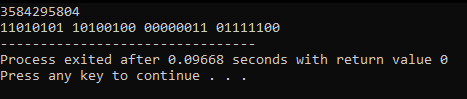
\includegraphics[scale=0.7]{infalaba1_0.png}
\label{image0}
\end{figure}

\clearpage
\item float $\rightarrow$ binary

\begin{lstlisting}[language=C++, basicstyle=\small]
union float_bin {
	float f;
	unsigned int i;
};

int main()
{	
	float a;
	float_bin fb;

	cin >> a;
	
	fb.f = a;

	print_bin(fb.i);

	return 0;
}
\end{lstlisting}

В данной задаче используется все та же функция print\char`_bin() из прошлого пункта. Для чтения побитового представления числа с плавающей точкой создадим объект union float\char`_bin. Сохраним в него float, и передадим его в функцию как unsigned int.

Пример работы:

\begin{figure}[h]
\centering
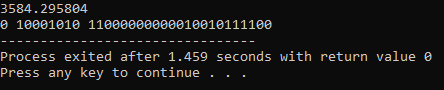
\includegraphics[scale=0.7]{infalaba1_1.png}
\label{image1}
\end{figure}

\clearpage
\item Переполнение мантиссы

\begin{lstlisting}[language=C++, basicstyle=\small]
int main() {	
	float a = 1;
	float_bin fb;
	
	cout << fixed;
	cout.precision(2);
	
	for (int i = 0; i < 40; i++) {
		cout << i << ' ' << a << endl;
		
		fb.f = a;
		print_bin(fb.i);
		
		cout << endl << endl;
			
		a *= 10;
	}

	return 0;
}
\end{lstlisting}

Используя функцию print\char`_bin() и структуру float\char`_bin, будем выводить на экран побитовое разложение числа с плавающей точкой, увеличивая его в 10 раз на каждой итерации. При переходе с $10^{10}$ до $10^{11}$, в переменную записывается число, отличное от ожидаемого результата. Это связано с дискретностью типа float. На 39 итерации переменная принимает значение inf.

Пример работы:

\begin{figure}[h]
\centering
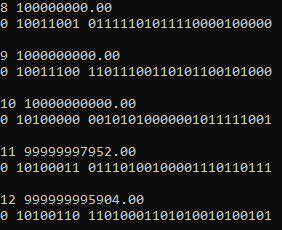
\includegraphics[scale=0.7]{infalaba1_2_1.png}
\label{image2_1}
\end{figure}

\begin{figure}[h]
\centering
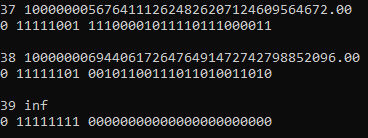
\includegraphics[scale=0.7]{infalaba1_2_2.png}
\label{image2_2}
\end{figure}

\clearpage
\item Бесконечный цикл

\begin{lstlisting}[language=C++, basicstyle=\small]
#include <iostream>
using namespace std;

int main()
{	
	cout << fixed;
	cout.precision(0);

	for (float i = 0; i <= 20000000; i++) {
		if (i + 1 == i) { 
			cout << i << endl;
		}
	}

	return 0;
}
\end{lstlisting}

Напишем данную программу. Условие, при котором цикл станет бесконечным, выполнится при $i=16777216=2^{24}$. Число $i + 1=16777217$ не может быть представлено переменной типа float.

\clearpage
\item График $\pi$

Для нахождения значения числа $\pi$ я выбрал 4 формулы:

\begin{enumerate}

\item $\frac{1}{1}-\frac{1}{3}+\frac{1}{5}-\frac{1}{7}+\frac{1}{9}-...=\frac{\pi}{4}$

\item $\frac{1}{1^2}+\frac{1}{2^2}+\frac{1}{3^2}+\frac{1}{4^2}+\frac{1}{5^2}+...=\frac{\pi^2}{6}$

\item $\frac{1}{1^2}-\frac{1}{2^2}+\frac{1}{3^2}-\frac{1}{4^2}+\frac{1}{5^2}-...=\frac{\pi^2}{12}$

\item $\sum_{k=0}^{\infty}\frac{(-1)^k}{3^k(2k+1)}=\frac{\pi}{2\sqrt{3}}$

\end{enumerate}

Ниже приведен код, вычисляющий $\pi$ по формуле (с).

\begin{lstlisting}[language=C++, basicstyle=\small]
#include <iostream>
#include <fstream>
#include <cmath>
using namespace std;

int main()
{	
	ofstream f("4_3.txt", ios::out);
	f << fixed;
	f.precision(22);
	
	float pi = 0, t, n;
	
	for (int i = 1; i < 10001; i++) {
		n = i;
		t = (i % 2 * 2 - 1);
		t = t / n / n;
		pi += t;
		f << i << '\t' << sqrt(pi * 12) << endl; 
	}
	return 0;
}
\end{lstlisting}

С помощью библиотеки matplotlib, построим график зависимости значения вычисленного числа $\pi$ от количества итераций.

\begin{figure}[h]
\centering

\includegraphics[scale=0.48]{infalaba1_4.png}
\label{image4}
\end{figure}

\clearpage
\item Время $\pi$

Преобразуем скрипт из прошлого пункта так, чтобы в файл записывалось время и номер итерации при которых вычисляется каждая цифра числа $\pi$. Пример опять же приведу только для пункта (c):

\begin{lstlisting}[language=C++, basicstyle=\small]
#include <iostream>
#include <cmath>
#include <fstream>
#include <chrono>
using namespace std;

int PI[12] = {3, 1, 4, 1, 5, 9, 2, 6, 5, 3, 5, 9};

int main()
{
	ofstream f("5_3.txt", ios::out);

	f << fixed;
	f.precision(22);

	cout << fixed;
	cout.precision(22);

	float pi = 0, t, n;
	int dn = 0;
	unsigned long int d = 0, ten = 1;

	auto start = chrono::high_resolution_clock::now();

	for (int i = 1; i < 100001; i++) {
		n = i;

		t = (i % 2 * 2 - 1);
		t /= n * n;

		pi += t;

		d = sqrt(pi * 12) * ten;
		d %= 10;

		if (d == PI[dn]) {
			auto end = std::chrono::high_resolution_clock::now();
			int time = (end - start).count();
			f << dn + 1 << '\t' << i << '\t' << time << endl;
			cout << i << '\t' << dn + 1 << '\t' <<
			sqrt(pi * 12) << '\t' << time << endl;

			dn++;
			ten *= 10;
		}
	}
	return 0;
}
\end{lstlisting}

По полученным данным построим два графика -- количество цифр числа $\pi$ в зависимости от количества итераций и в зависимости от времени.

\begin{figure}[h]
\centering
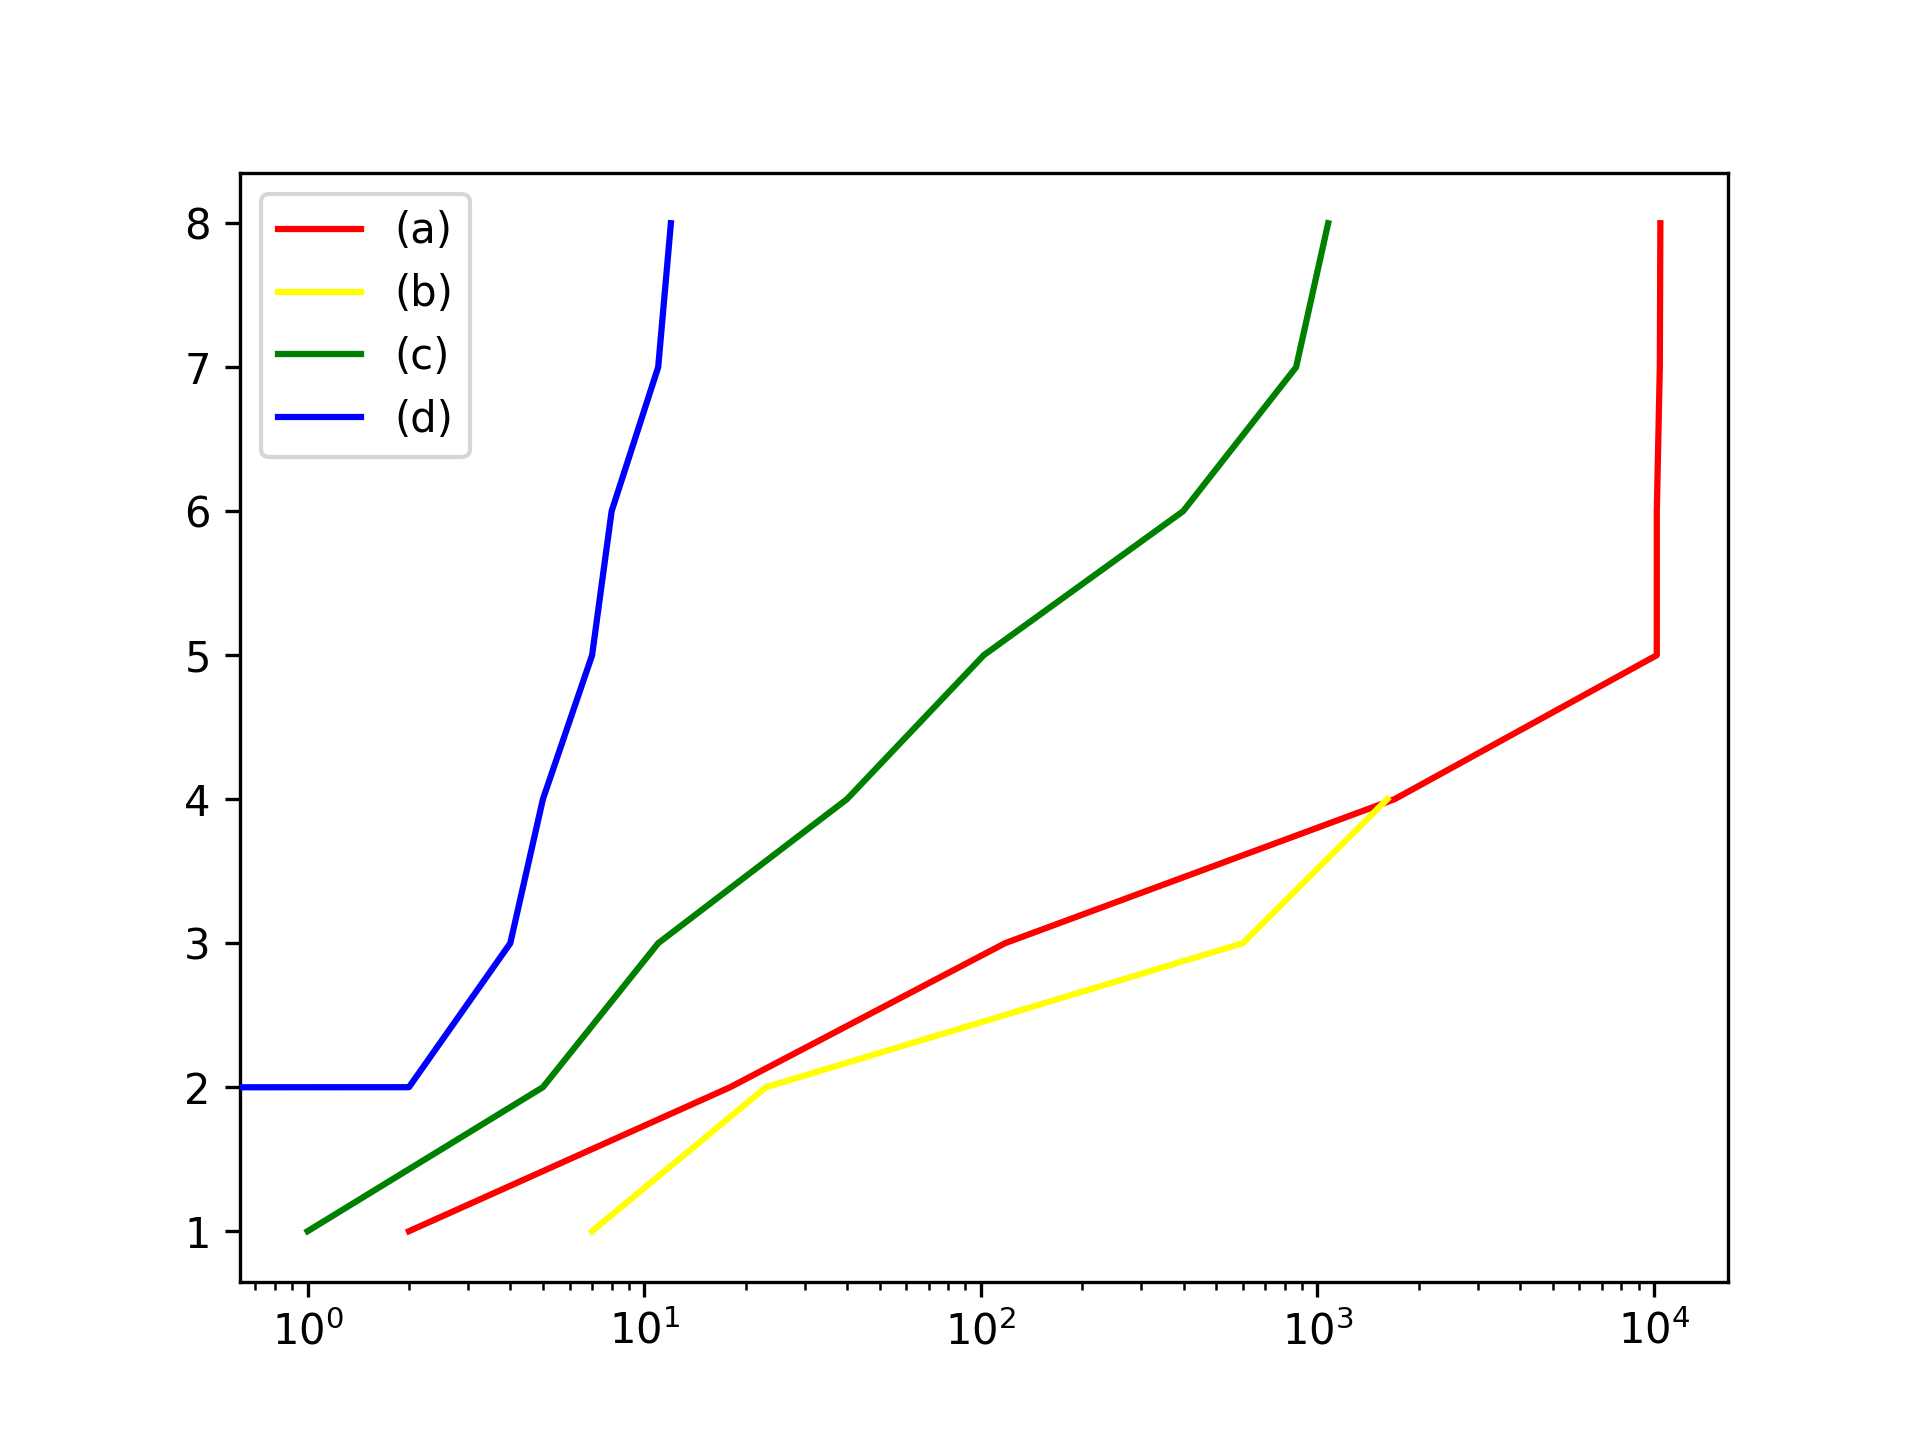
\includegraphics[scale=0.6]{infalaba1_5_1.png}
\label{image5_1}
\end{figure}

\begin{figure}[h]
\centering
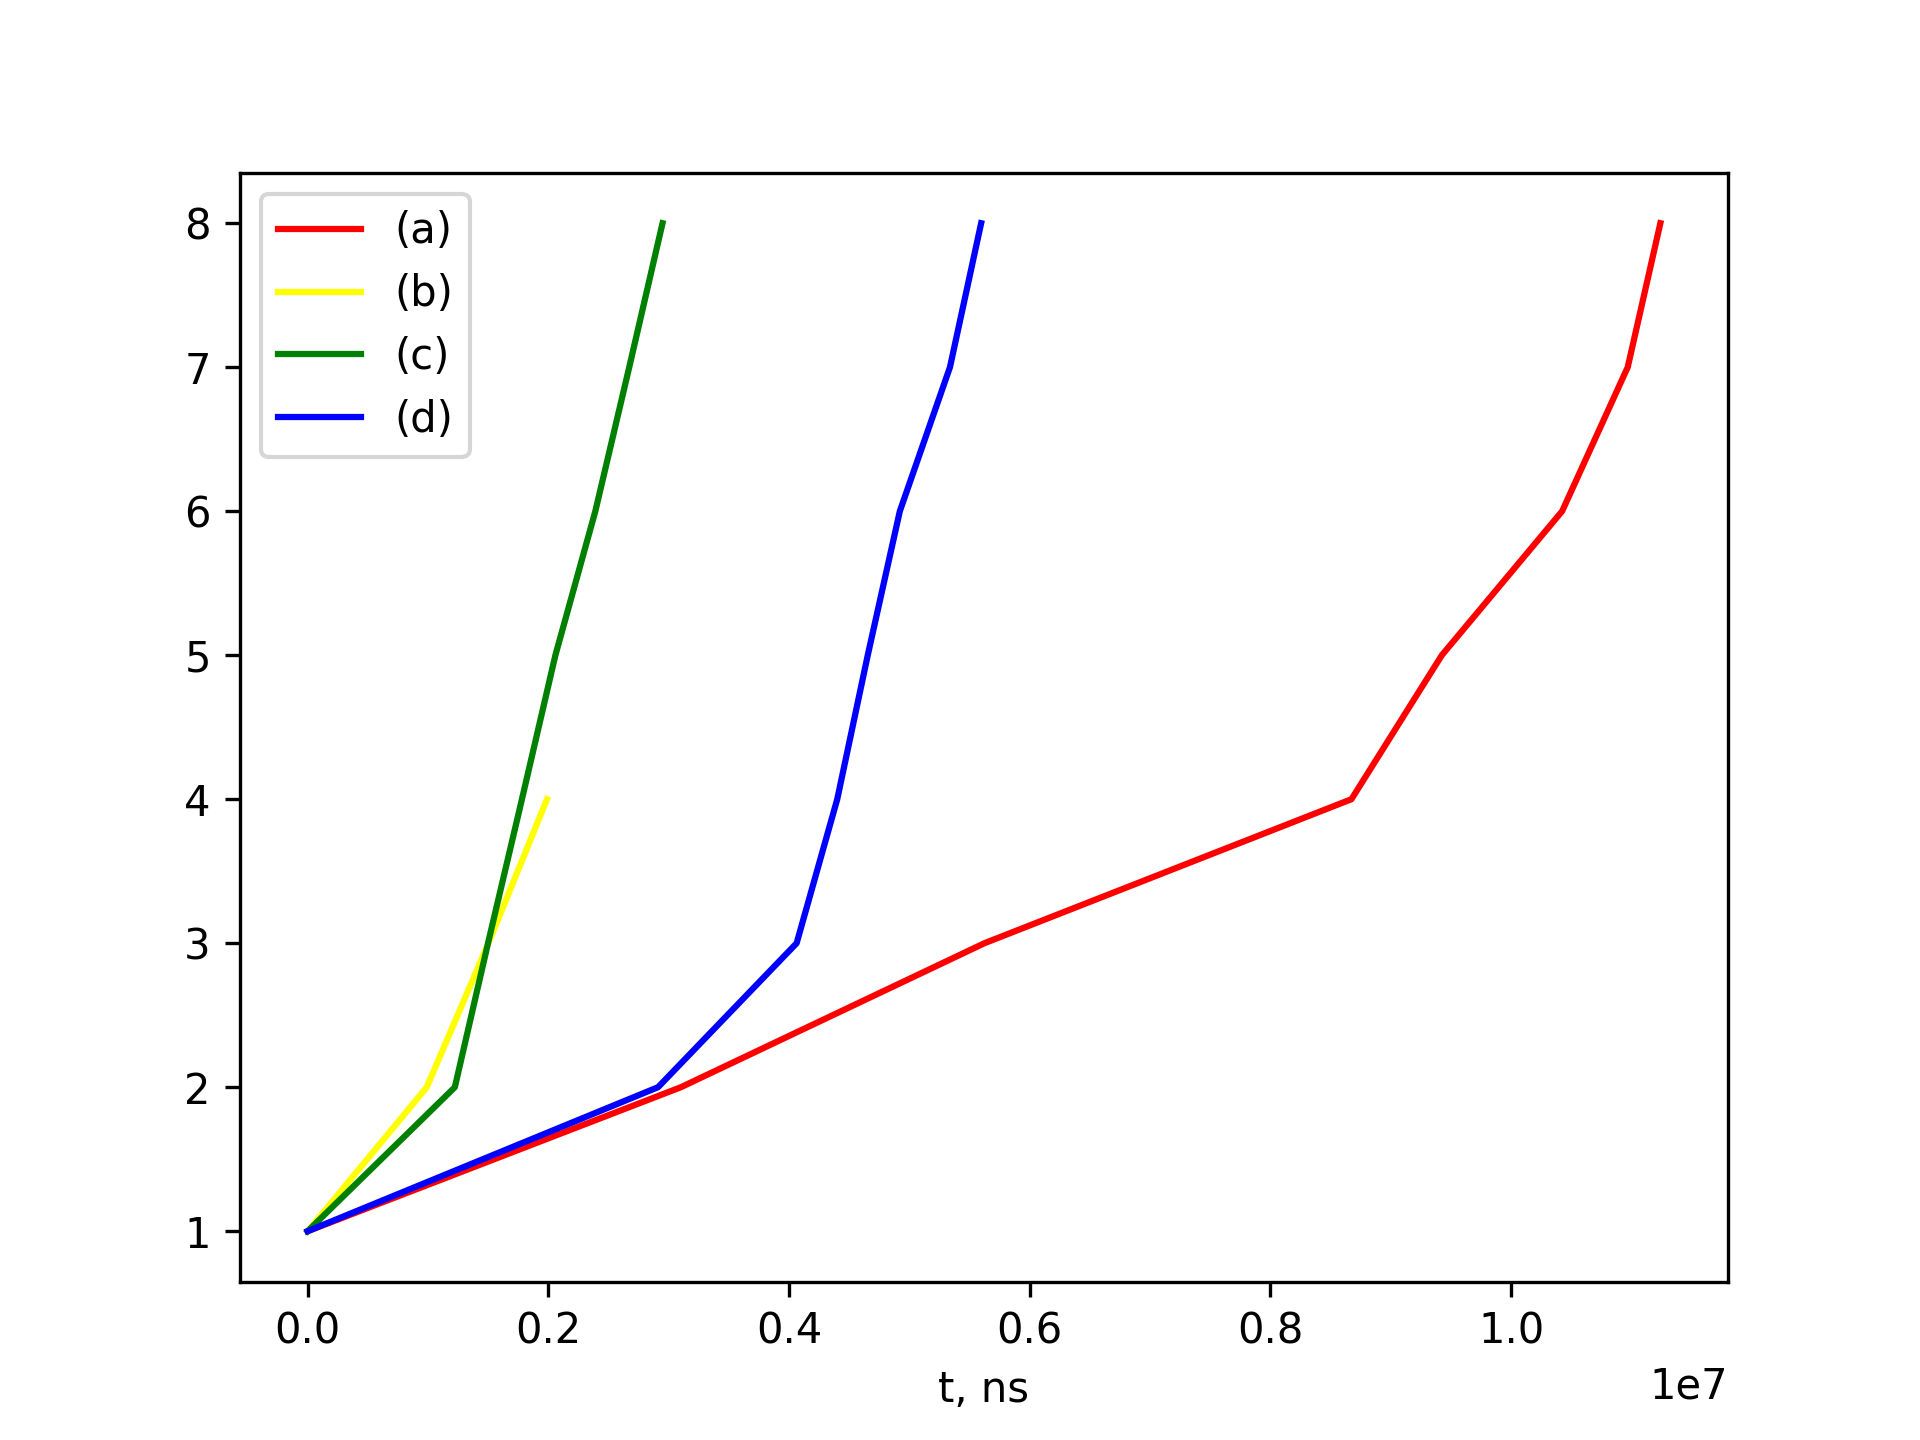
\includegraphics[scale=0.6]{infalaba1_5_2.png}
\label{image5_2}
\end{figure}

\end{enumerate}

\end{document}